\section{IoT}
En esta seccion se demostrara como usar el Azure Sphere para conectarse al servicio Azure IoT Hub de Microsoft.
\subsection{Registro en Azure}
Registre una cuenta gratuita en \href{https://azure.microsoft.com/es-mx/free}{Azure}. Para esto,	 necesita obligatoriamente un numero telefónico y una tarjeta de crédito o débito para verificar su identidad.

Ahora se tiene que crear un IoT Hub, este es un servicio de la nube que funciona como un centro de comunicación entre distintos aplicaciones IoT. Para crearlo, en el panel de Azure, selecciona Create a resource.
\begin{figure}[h]
	\centering
	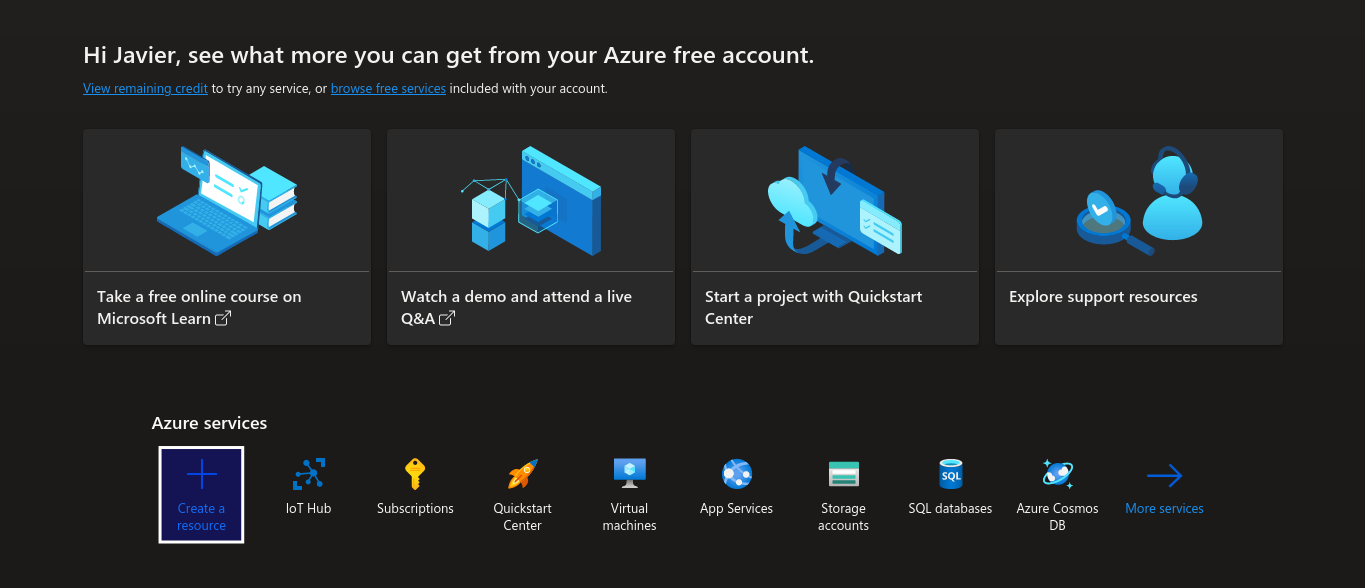
\includegraphics[width=0.75\textwidth,height=\textheight,keepaspectratio]{Azure1}
	\caption{Página de inicio de Azure.}
\end{figure}

En la página de ``Create a resource'', en la sección de categorías, elige Internet of Things y presiona IoT Hub.
\begin{figure}[h]
	\centering
	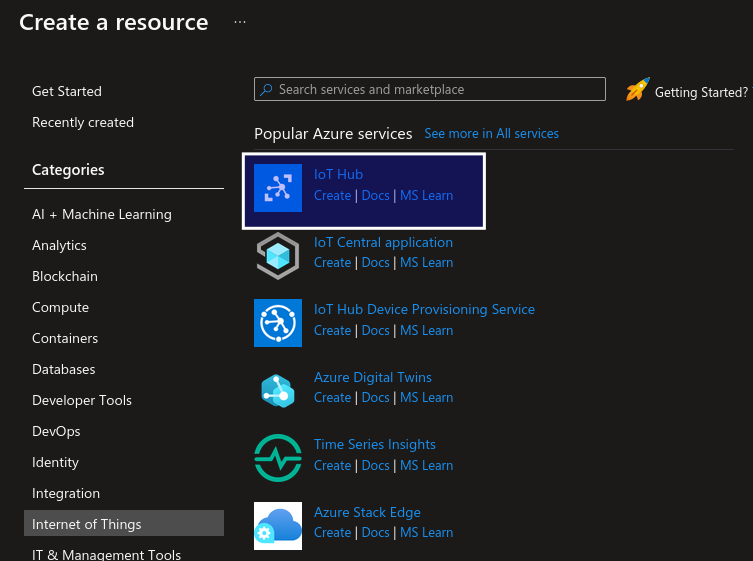
\includegraphics[width=0.70\textwidth,height=\textheight,keepaspectratio]{Azure2}
	\caption{Sección de crear recursos.}
\end{figure}

Llena todos los datos para el registro de tu \textbf{IoT Hub}. El \textbf{resource group} lo puedes crear ahí mismo. La región elige la de tu preferencia. El nivel elige gratuito. El nombre del Hub solo tienen que ser letras. Al tener todo listo da clic en \textbf{review + create} y para confirmar \textbf{create}.
\begin{figure}[h]
	\centering
	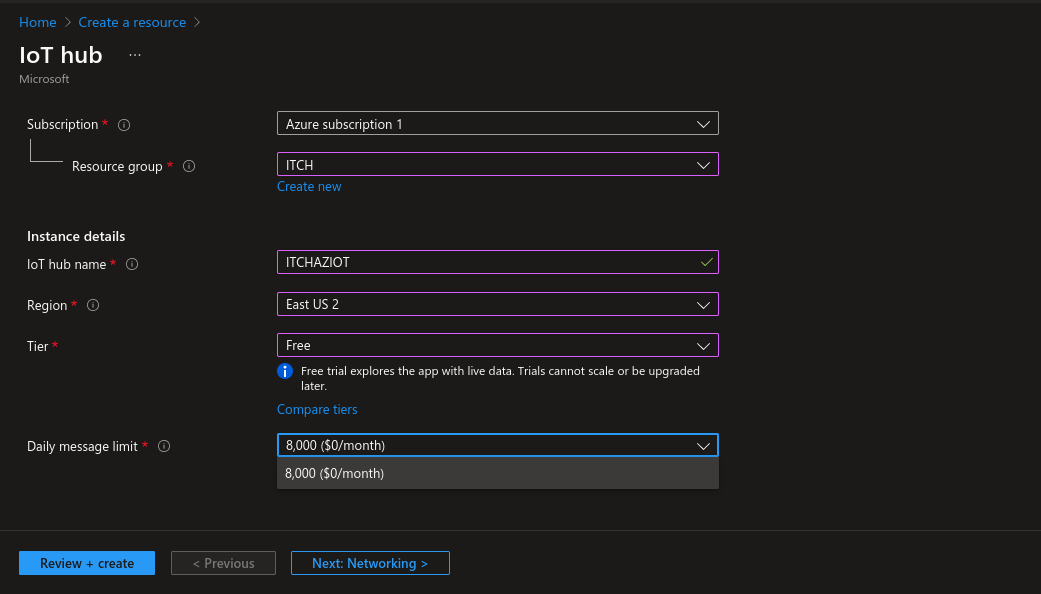
\includegraphics[width=0.75\textwidth,height=\textheight,keepaspectratio]{Azure3}
	\caption{Formulario para la creación de un IoT Hub.}
\end{figure}

\subsection{Certificado del Azure Sphere}
Con el objetivo de tener una correcta comunicación entre el dispositivo y el centro IoT se necesita generar un certificado.

En la terminal, ejecutar el siguiente comando.
\begin{verbatim}
	azsphere ca-certificate download --destination CAcertificate.cer
\end{verbatim}
Esto generara un certificado en el directorio que se encuentre la terminal.
\pagebreak
\subsection{Subir el certificado al IoT hub}
Navega al IoT hub que creaste.
\begin{figure}[h]
	\centering
	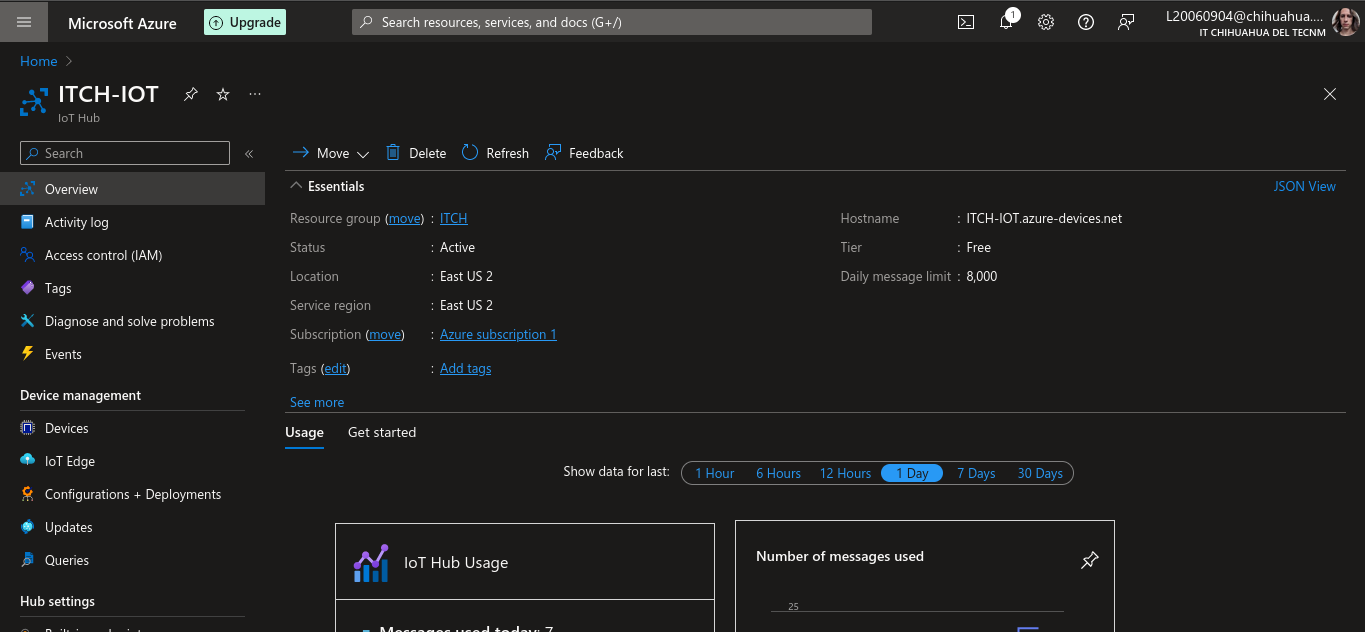
\includegraphics[width=0.75\textwidth,height=\textheight,keepaspectratio]{Azure4}
	\caption{Descripción general del IoT Hub.}
\end{figure}

Ve a la sección de certificados.
\begin{figure}[h]
	\centering
	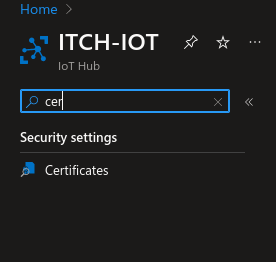
\includegraphics[width=0.75\textwidth,height=0.35\textheight,keepaspectratio]{Azure5}
	\caption{Búsqueda del apartado certificados.}
\end{figure}

\pagebreak
Ya estando en la sección, presiona el botón de add.
\begin{figure}[h]
	\centering
	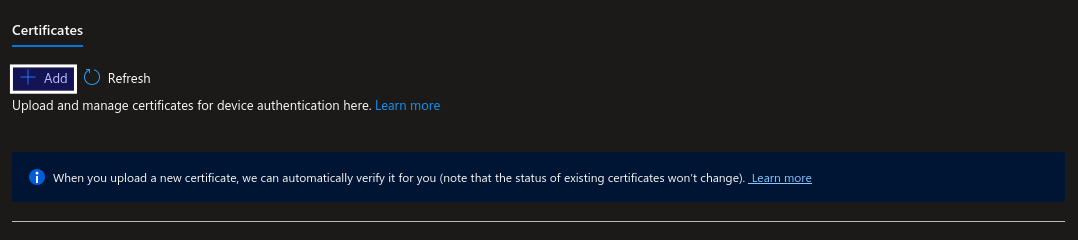
\includegraphics[width=0.9\textwidth,height=\textheight,keepaspectratio]{Azure6}
	\caption{Sección de certificados.}
\end{figure}

Agrega el nombre, el archivo del certificado y marca la casilla de "Set certificate status to verified on upload".
\begin{figure}[h]
	\centering
	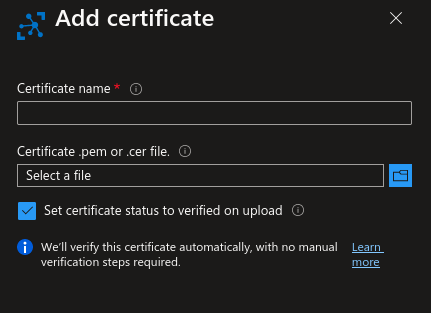
\includegraphics[width=0.9\textwidth,height=\textheight,keepaspectratio]{Azure7}
	\caption{Solicitud del certificado.}
\end{figure}
\pagebreak
\subsection{Agregar dispositivo}
En la pagina del IoT Hub, navega a la sección de dispositivos.
\begin{figure}[h]
	\centering
	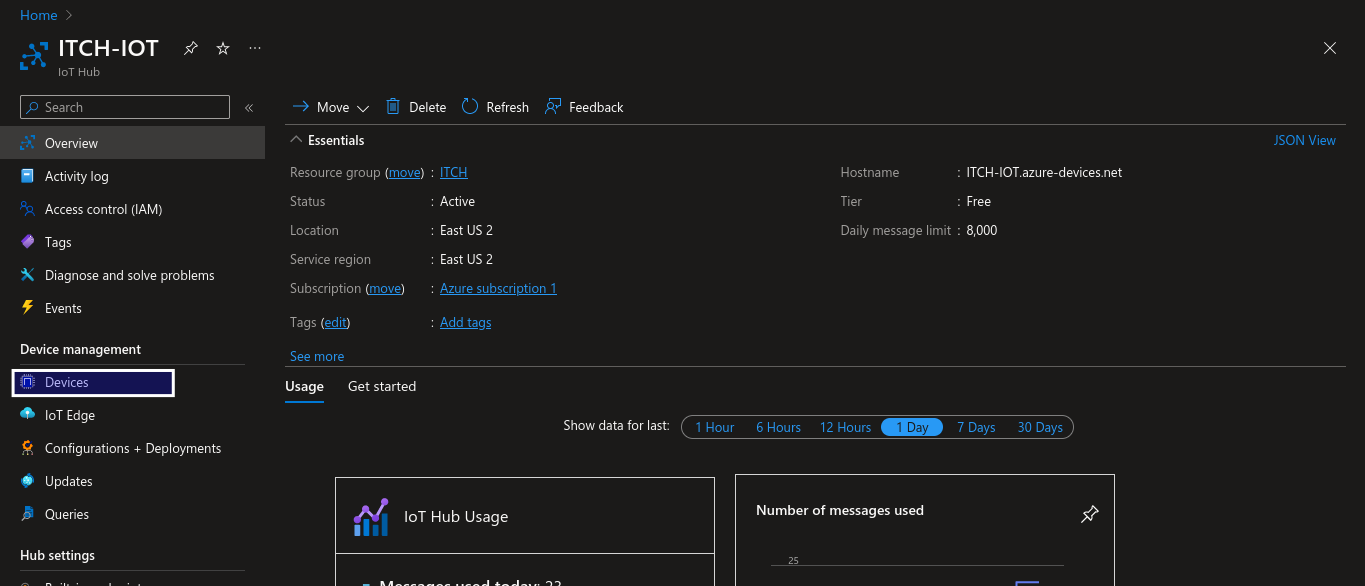
\includegraphics[width=0.75\textwidth,height=\textheight,keepaspectratio]{Azure8}
	\caption{Descripción general del IoT Hub.}
\end{figure}

Estando en la sección, presiona el botón de add device
\begin{figure}[h]
	\centering
	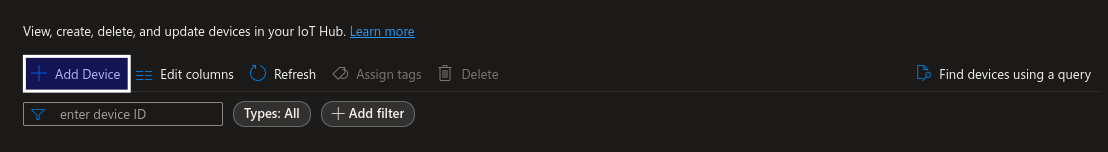
\includegraphics[width=0.9\textwidth,height=\textheight,keepaspectratio]{Azure9}
	\caption{Sección de dispositivos.}
\end{figure}

\pagebreak
Agrega el id del dispositivo, este lo obtienes en la terminal con el siguiente comando (El dispositivo debe estar conectado a la computadora):
\begin{verbatim}
	azsphere device show-attached
\end{verbatim}
En el tipo de autenticación eliges X.509 CA Signed. Despues presiona save.
\begin{figure}[h]
	\centering
	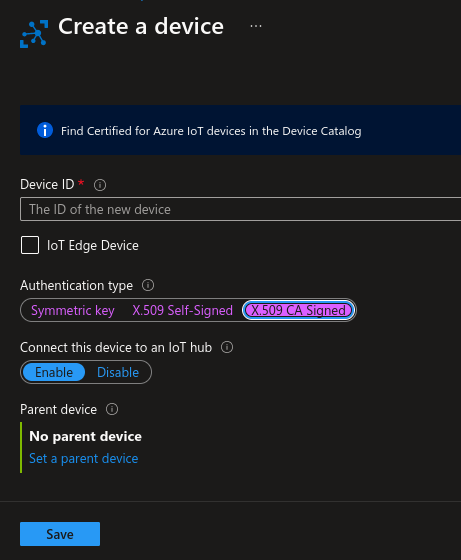
\includegraphics[width=0.70\textwidth,height=\textheight,keepaspectratio]{Azure10}
	\caption{Formulario del dispositivo.}
\end{figure}
